% !TeX spellcheck = en_GB
\documentclass[10pt,aspectratio=169,usenames,dvipsnames]{beamer}

\usetheme[block=fill,progressbar=frametitle]{metropolis}
\usepackage{appendixnumberbeamer}
\usepackage{booktabs}
\usepackage{siunitx}
\usepackage{fontspec}
\defaultfontfeatures{Extension = .otf}
\usepackage{fontawesome5}
\usepackage{pgfplots}

\title{Multipoint observations of ICMEs\\in the inner heliosphere}
\subtitle{Forbush decreases and remote sensing}
\author{Johan L. Freiherr von Forstner\\IEAP, Christian-Albrechts-Universität zu Kiel}
\date{Disputation --- 16.02.2020}
\titlegraphic{\hfill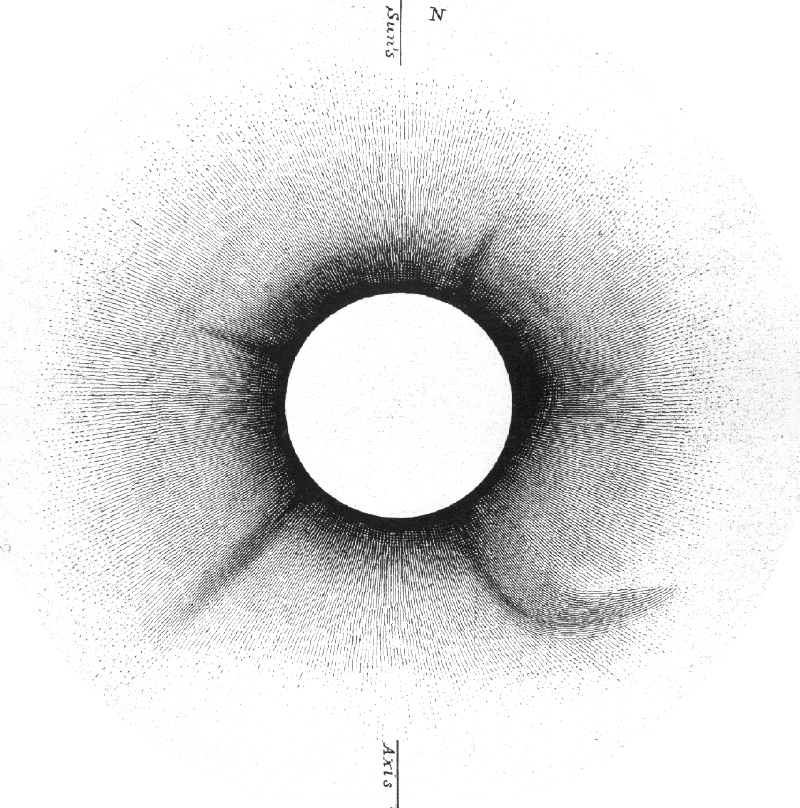
\includegraphics[height=3.6cm]{../images/oldcme3_inverted.png}}

% Color scheme
\definecolor{mOrange}{HTML}{FF9400} % Math-Nat-Fakultät
\definecolor{mBlue}{HTML}{0B5FA5}
\definecolor{mBlueDark}{HTML}{053964}
\definecolor{mGreen}{HTML}{00AE68}
\setbeamercolor{normal text}{fg=black, bg=white}
\setbeamercolor{palette primary}{bg=mBlueDark, fg=white}
\setbeamercolor{frametitle}{bg=mOrange, fg=black}
\setbeamercolor{alerted text}{fg=mOrange}
\setbeamercolor{example text}{fg=mGreen}
\setbeamercolor{progress bar}{fg=mBlue,bg=black!10}

\usepackage[absolute,overlay]{textpos}

\setbeamercolor{framesource}{fg=gray}
\setbeamerfont{framesource}{size=\tiny}

\usetikzlibrary{calc}
\usetikzlibrary{decorations.pathmorphing,decorations.markings,pgfplots.fillbetween}
\definecolor{red}{HTML}{d62728}
\definecolor{orange}{HTML}{ff7f0e}
\definecolor{green}{HTML}{2ca02c}
\definecolor{blue}{HTML}{1f77b4}
\definecolor{purple}{HTML}{9467bd}
\definecolor{light-gray}{gray}{0.9}

% siunitx setup
\sisetup{detect-family=true, mode=text, range-units=single, separate-uncertainty=true}
\DeclareSIUnit\AU{AU}
\DeclareSIUnit\astronomicalunit{AU}
\DeclareSIUnit\solarradius{\ensuremath{R_{\astrosun}}}

\begin{document}
\maketitle

\begin{frame}{Contents}
    \tableofcontents
\end{frame}

\section{Introduction}

\begin{frame}
    Inhalt...
\end{frame}

\begin{frame}{Observation of (I)CMEs}
    \begin{columns}
        \begin{column}{0.45\textwidth}
            \textbf{In situ}
        \end{column}
        \begin{column}{0.45\textwidth}
            \textbf{Remote sensing}
        \end{column}
    \end{columns}
\end{frame}

\begin{frame}{Ideal constellations for multipoint (I)CME observations}
    \vspace{3mm}
    \begin{columns}
        \begin{column}{0.45\textwidth}
            \textbf{In situ:} \uncover<2->{regular grid of observers}\\[0.2cm]
            \centering
            \begin{tikzpicture}
                \def\earthorbitradius{2.5}
                \def\sunradius{0.2}
                
                % CME
                \def\cmeangle{45}	
                \def\cmeheight{2}	
                \draw[name path=CMEin] (\cmeangle-30:\sunradius) % inner edge
                .. controls (\cmeangle-45:\sunradius*3*\cmeheight) and +(\cmeangle - 90:\sunradius*0.7*\cmeheight) ..
                (\cmeangle:\sunradius*3*\cmeheight)
                .. controls +(\cmeangle + 90:\sunradius*0.7*\cmeheight) and (\cmeangle+45:\sunradius*3*\cmeheight) ..
                (\cmeangle+30:\sunradius);
                
                \draw[name path=CMEout] (\cmeangle-40:\sunradius) % outer edge
                .. controls (\cmeangle-55:\sunradius*3*\cmeheight) and +(\cmeangle - 90:\sunradius*2*\cmeheight) ..
                (\cmeangle:\sunradius*4*\cmeheight)
                .. controls +(\cmeangle + 90:\sunradius*2*\cmeheight) and (\cmeangle+55:\sunradius*3*\cmeheight) ..
                (\cmeangle+40:\sunradius);
                
                \tikzfillbetween[of=CMEout and CMEin]{orange, opacity=0.1};
                           
                % sun
                \draw[fill=yellow] (0, 0) circle (\sunradius);
                
                % Earth
                \draw[dashed] (0, 0) circle (\earthorbitradius);
                \draw[fill=blue] (45:\earthorbitradius) circle (0.1);
                
                % satellites
                \uncover<2->{
                    \node at (45:0.25*\earthorbitradius) {\faSatellite};
                    \node at (45:0.5*\earthorbitradius) {\faSatellite};
                    \node at (45:0.75*\earthorbitradius) {\faSatellite};
                }
                
                \uncover<3->{
                \foreach \angle in {0,90,135,180,225,270,315,360} {
                    \node[rotate={\angle-45}] at (\angle:0.25*\earthorbitradius) {\faSatellite};
                    \node[rotate={\angle-45}] at (\angle:0.5*\earthorbitradius) {\faSatellite};
                    \node[rotate={\angle-45}] at (\angle:0.75*\earthorbitradius) {\faSatellite};
                    \node[rotate={\angle-45}] at (\angle:\earthorbitradius) {\faSatellite};
                }}
            \end{tikzpicture}
        \end{column}
        \begin{column}{0.45\textwidth}
            \textbf{Remote sensing:} \uncover<4->{from the side}\\[0.2cm]
            \centering
            \begin{tikzpicture}
                \def\earthorbitradius{2.5}
                \def\sunradius{0.2}
                
                % CME
                \def\cmeangle{45}	
                \def\cmeheight{2}	
                \draw[name path=CMEin] (\cmeangle-30:\sunradius) % inner edge
                .. controls (\cmeangle-45:\sunradius*3*\cmeheight) and +(\cmeangle - 90:\sunradius*0.7*\cmeheight) ..
                (\cmeangle:\sunradius*3*\cmeheight)
                .. controls +(\cmeangle + 90:\sunradius*0.7*\cmeheight) and (\cmeangle+45:\sunradius*3*\cmeheight) ..
                (\cmeangle+30:\sunradius);
                
                \draw[name path=CMEout] (\cmeangle-40:\sunradius) % outer edge
                .. controls (\cmeangle-55:\sunradius*3*\cmeheight) and +(\cmeangle - 90:\sunradius*2*\cmeheight) ..
                (\cmeangle:\sunradius*4*\cmeheight)
                .. controls +(\cmeangle + 90:\sunradius*2*\cmeheight) and (\cmeangle+55:\sunradius*3*\cmeheight) ..
                (\cmeangle+40:\sunradius);
                
                \tikzfillbetween[of=CMEout and CMEin]{orange, opacity=0.1};
                
                % sun
                \draw[fill=yellow] (0, 0) circle (\sunradius);
                
                % Earth
                \draw[dashed] (0, 0) circle (\earthorbitradius);
                \draw[fill=blue] (45:\earthorbitradius) circle (0.1);
                
                % satellites
                \uncover<4->{
                    \node[rotate=90] at (135:\earthorbitradius) {\faSatellite};
                    \node[rotate=-90] at (-45:\earthorbitradius) {\faSatellite};
                    \draw (135:\earthorbitradius) -- ++(-9:3.5);
                    \draw (-45:\earthorbitradius) -- ++(99:3.5);
                }
                    
                \uncover<5->{
                \foreach \angle in {0,45,90,180,225,270,360} {
                    \node[rotate={\angle-45}] at (\angle:\earthorbitradius) {\faSatellite};
                }}
            \end{tikzpicture}
        \end{column}
    \end{columns}
    \centering
    \uncover<6->{\textbf{Unrealistic.} So what can we do with existing spacecraft?}
    \begin{flushright}
        \footnotesize not to scale
    \end{flushright}
    
\end{frame}

\begin{frame}{Fleet of heliophysics missions}
    \vspace{3mm}
    \begin{columns}
        \begin{column}{0.45\textwidth}
            \textbf{In situ}\\[0.2cm]
            \centering
            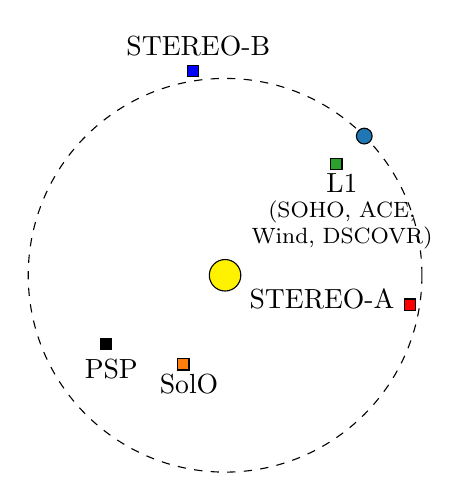
\begin{tikzpicture}
                \def\earthorbitradius{2.5}
                \def\sunradius{0.2}
                
                % sun
                \draw[fill=yellow] (0, 0) circle (\sunradius);
                
                % Earth
                \draw[dashed] (0, 0) circle (\earthorbitradius);
                \draw[fill=blue] (45:\earthorbitradius) circle (0.1);
                
                % satellites
                \draw[fill=Blue] ({45+54}:1.05*\earthorbitradius) +(-2pt,-2pt) rectangle +(2pt,2pt) node[above] {STEREO-B};
                \draw[fill=Red] ({45-54}:0.95*\earthorbitradius) +(-2pt,-2pt) rectangle +(2pt,2pt) node[left, xshift=-4pt] {STEREO-A};
                
                \draw[fill=green] (45:0.8*\earthorbitradius) +(-2pt,-2pt) rectangle +(2pt,2pt) node[below, yshift=-2pt, align=center] {L1\\[-1mm]\footnotesize (SOHO, ACE,\\[-1mm]\footnotesize Wind, DSCOVR)};
                
                \draw[fill=orange] (245:0.5*\earthorbitradius) +(-2pt,-2pt) rectangle +(2pt,2pt) node[below, yshift=-2pt] {SolO};
                \draw[fill=black] (210:0.7*\earthorbitradius) +(-2pt,-2pt) rectangle +(2pt,2pt) node[below, yshift=-4pt] {PSP};
                
            \end{tikzpicture}
        \end{column}
        \begin{column}{0.45\textwidth}
            \textbf{Remote sensing}\\[0.2cm]
            \centering
            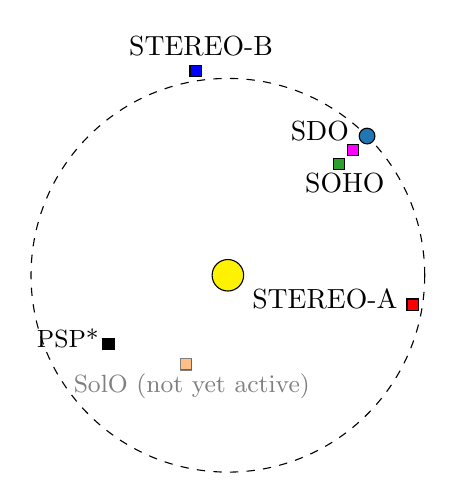
\begin{tikzpicture}
                \def\earthorbitradius{2.5}
                \def\sunradius{0.2}
                
                % sun
                \draw[fill=yellow] (0, 0) circle (\sunradius);
                
                % Earth
                \draw[dashed] (0, 0) circle (\earthorbitradius);
                \draw[fill=blue] (45:\earthorbitradius) circle (0.1);
                
                \draw[fill=Blue] ({45+54}:1.05*\earthorbitradius) +(-2pt,-2pt) rectangle +(2pt,2pt) node[above] {STEREO-B};
                \draw[fill=Red] ({45-54}:0.95*\earthorbitradius) +(-2pt,-2pt) rectangle +(2pt,2pt) node[left, xshift=-4pt] {STEREO-A};
                
                \draw[fill=Magenta] (45:0.9*\earthorbitradius) +(-2pt,-2pt) rectangle +(2pt,2pt) node[above left,yshift=-2pt] {SDO};
                \draw[fill=green] (45:0.8*\earthorbitradius) +(-2pt,-2pt) rectangle +(2pt,2pt) node[below,yshift=-2pt] {SOHO};
                
                \draw[fill=orange,opacity=0.5] (245:0.5*\earthorbitradius) +(-2pt,-2pt) rectangle +(2pt,2pt) node[below, yshift=-2pt] {\small SolO (not yet active)};
                \draw[fill=black] (210:0.7*\earthorbitradius) +(-2pt,-2pt) rectangle +(2pt,2pt) node[left, xshift=-2pt] {\small PSP*};
               
            \end{tikzpicture}
        \end{column}
    \end{columns}
    \begin{flushright}
        \footnotesize not to scale
    \end{flushright}
\end{frame}

\section{Instrumentation}

\begin{frame}{MSL/RAD}
    \begin{columns}
        \begin{column}{0.45\textwidth}
            
        \end{column}
        \begin{column}{0.45\textwidth}
            %\documentclass{standalone}
%\usepackage{tikz}
%\usepackage{amsmath}

%\usetikzlibrary{calc}
%\usetikzlibrary{decorations.pathmorphing}

%\definecolor{light-gray}{gray}{0.9}

%\begin{document}
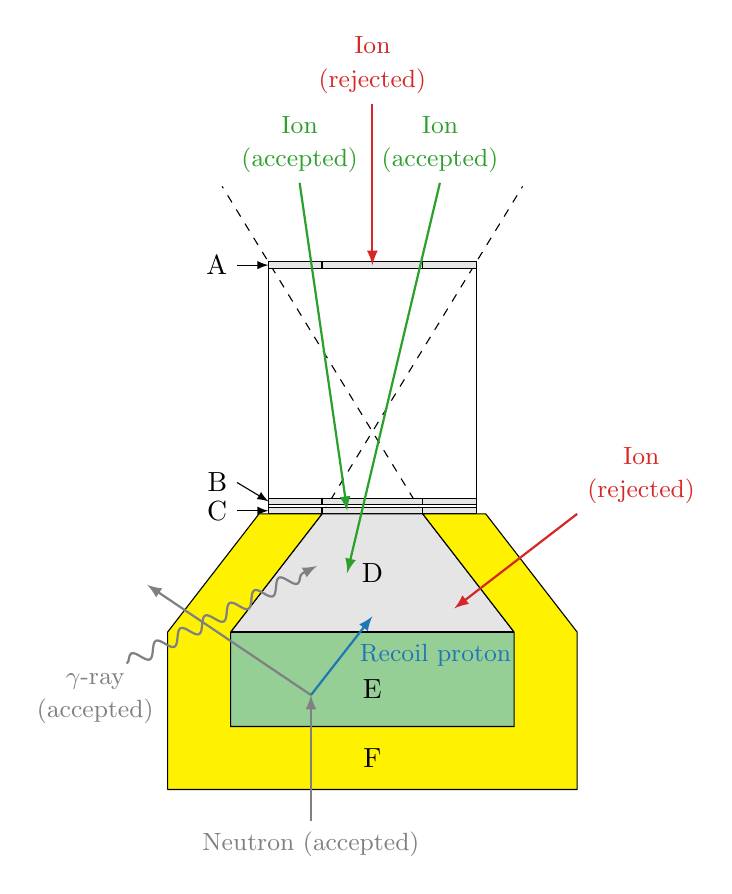
\begin{tikzpicture}[scale=0.8]
    \tikzset{%
        add/.style args={#1 and #2}{
            to path={%
                ($(\tikztostart)!-#1!(\tikztotarget)$)--($(\tikztotarget)!-#2!(\tikztostart)$)%
                \tikztonodes},add/.default={.2 and .2}}
    }  
    
    \def\bottomwidth{3.25}
    \def\midwidth{1.8}
    \def\topwidth{1.65}
    \def\bottomheight{2.5}
    \def\midheight{4.375}
    \def\Fthickness{1}
    \def\Sithickness{0.1}
    \def\BCdistance{0.15}
    \def\topheight{8.375}
    
    % FOV
    \draw[add=0 and 0.3, dashed] (\midwidth - \Fthickness, \midheight) to (-\topwidth, \topheight);
    \draw[add=0 and 0.3, dashed] (-\midwidth + \Fthickness, \midheight) to (\topwidth, \topheight);

    % A
    \draw[fill=light-gray] (-\topwidth, \topheight - \Sithickness) rectangle (\topwidth, \topheight);
    \draw (-\midwidth + \Fthickness, \topheight - \Sithickness) --  (-\midwidth + \Fthickness, \topheight);
    \draw (-\midwidth + \Fthickness, \topheight - \Sithickness) --  (-\midwidth + \Fthickness, \topheight);
    \draw (\midwidth - \Fthickness, \topheight - \Sithickness) --  (\midwidth - \Fthickness, \topheight);
    \draw (\midwidth - \Fthickness, \topheight - \Sithickness) --  (\midwidth - \Fthickness, \topheight);
    \draw[latex-] (-\topwidth, \topheight - \Sithickness / 2) -- (-\topwidth - 0.5, \topheight - \Sithickness / 2) node[left] {A};
    
    % B
    \draw[fill=light-gray] (-\topwidth, \midheight + \BCdistance) rectangle (\topwidth, \midheight + \BCdistance + \Sithickness);
    \draw (-\midwidth + \Fthickness, \midheight + \BCdistance) --  (-\midwidth + \Fthickness, \midheight + \BCdistance + \Sithickness);
    \draw (-\midwidth + \Fthickness, \midheight + \BCdistance) --  (-\midwidth + \Fthickness, \midheight + \BCdistance + \Sithickness);
    \draw (\midwidth - \Fthickness, \midheight + \BCdistance) --  (\midwidth - \Fthickness, \midheight + \BCdistance + \Sithickness);
    \draw (\midwidth - \Fthickness, \midheight + \BCdistance) --  (\midwidth - \Fthickness, \midheight + \BCdistance + \Sithickness);
    \draw[latex-] (-\topwidth, \midheight + \BCdistance + \Sithickness / 2) -- (-\topwidth - 0.5, \midheight + \BCdistance + \Sithickness / 2 + 0.3) node[left] {B};
    
    % C
    \draw[fill=light-gray] (-\topwidth, \midheight) rectangle (\topwidth, \midheight + \Sithickness);
    \draw (-\midwidth + \Fthickness, \midheight) --  (-\midwidth + \Fthickness, \midheight + \Sithickness);
    \draw (-\midwidth + \Fthickness, \midheight) --  (-\midwidth + \Fthickness, \midheight + \Sithickness);
    \draw (\midwidth - \Fthickness, \midheight) --  (\midwidth - \Fthickness, \midheight + \Sithickness);
    \draw (\midwidth - \Fthickness, \midheight) --  (\midwidth - \Fthickness, \midheight + \Sithickness);
    \draw[latex-] (-\topwidth, \midheight + \Sithickness / 2) -- (-\topwidth - 0.5, \midheight + \Sithickness / 2) node[left] {C};
    
    % border of ABC
    \draw (-\topwidth, \midheight) -- (-\topwidth, \topheight);
    \draw (\topwidth, \midheight) -- (\topwidth, \topheight);
    
    % D
    \draw[fill=light-gray] (\bottomwidth - \Fthickness, \bottomheight) --  (-\bottomwidth + \Fthickness, \bottomheight) -- (-\midwidth + \Fthickness, \midheight) -- (\midwidth - \Fthickness, \midheight) -- (\bottomwidth - \Fthickness, \bottomheight);   
    \node at (0, {\bottomheight + (\midheight - \bottomheight) / 2}) {D};   
    
    % E
    \draw[fill=green!50] (\bottomwidth - \Fthickness, \bottomheight) -- (\bottomwidth - \Fthickness, \Fthickness) --
    (-\bottomwidth + \Fthickness, \Fthickness) --  (-\bottomwidth + \Fthickness, \bottomheight) -- (\bottomwidth - \Fthickness, \bottomheight);  
    \node at (0, {\Fthickness + (\bottomheight - \Fthickness) * 0.4}) {E};   
    
    % F
    \draw[fill=yellow] (-\bottomwidth, 0) -- (\bottomwidth, 0) -- (\bottomwidth, \bottomheight) -- (\midwidth, \midheight) --
    (\midwidth - \Fthickness, \midheight) -- (\bottomwidth - \Fthickness, \bottomheight) -- (\bottomwidth - \Fthickness, \Fthickness) --
    (-\bottomwidth + \Fthickness, \Fthickness) --  (-\bottomwidth + \Fthickness, \bottomheight) -- (-\midwidth + \Fthickness, \midheight) --
    (-\midwidth, \midheight) -- (-\bottomwidth, \bottomheight) -- (-\bottomwidth, 0);     
    \node at (0, \Fthickness / 2) {F};
    
    % trajectories of ions
    \draw[thick, green, -latex] (-\topwidth*0.7, \topheight*1.15) node[above, align=center] {\small Ion\\ \small (accepted)}
     -- ({-(\midwidth - \Fthickness) * 0.5}, \midheight + \Sithickness / 2);
    \draw[thick, green, -latex] (\topwidth*0.65, \topheight*1.15) node[above, align=center] {\small Ion\\ \small (accepted)}
     -- ({-(\midwidth - \Fthickness) * 0.5}, {\bottomheight +  (\midheight - \bottomheight) / 2});
    \draw[thick, red, -latex] (0, \topheight*1.3) node[above, align=center] {\small Ion\\ \small (rejected)}
     -- (0, \topheight - \Sithickness / 2);
    \draw[thick, red, -latex] (\bottomwidth, \midheight) node[above right, align=center] {\small Ion\\ \small (rejected)}
    -- (\bottomwidth * 0.4, {\bottomheight + (\midheight - \bottomheight) * 0.2});
    
    % trajectory of neutron
    \draw[thick, gray, -latex] (-\bottomwidth*0.3, -0.5) node[below] {\small Neutron (accepted)}
    -- (-\bottomwidth*0.3, {\Fthickness + \bottomheight * 0.2});
    \draw[thick, gray, -latex]  (-\bottomwidth*0.3, {\Fthickness + \bottomheight * 0.2}) -- (-\bottomwidth * 1.1, \bottomheight * 1.3);
    \draw[thick, blue, -latex]  (-\bottomwidth*0.3, {\Fthickness + \bottomheight * 0.2}) -- (0, \bottomheight * 1.1) node[midway, right, xshift=1mm] {\small Recoil proton};
    
    % trajectory of gamma
    \draw[thick, gray, decorate, decoration=snake] (-\bottomwidth*1.2, \bottomheight * 0.8) node[below, align=center, xshift=-4mm] {\small $\gamma$-ray\\ \small (accepted)} -- (-\bottomwidth * 0.3, \bottomheight * 1.4);
    \draw[thick, gray, -latex] (-\bottomwidth * 0.3, \bottomheight * 1.4) -- ++ (\bottomwidth * 0.03, \bottomheight * 0.02);
    
\end{tikzpicture}
%\end{document}
        \end{column}
    \end{columns}
\end{frame}

\begin{frame}{Solar Orbiter HET}
    \begin{columns}
        \begin{column}{0.25\textwidth}
            
        \end{column}
        \begin{column}{0.65\textwidth}
            %\documentclass{standalone}
%\usepackage[dvipsnames]{xcolor}
%\usepackage{tikz}
%\usepackage{amsmath}
%\usepackage{siunitx}

%\usetikzlibrary{calc}
%\usetikzlibrary{decorations.pathmorphing}

%\definecolor{light-gray}{gray}{0.9}

%\begin{document}
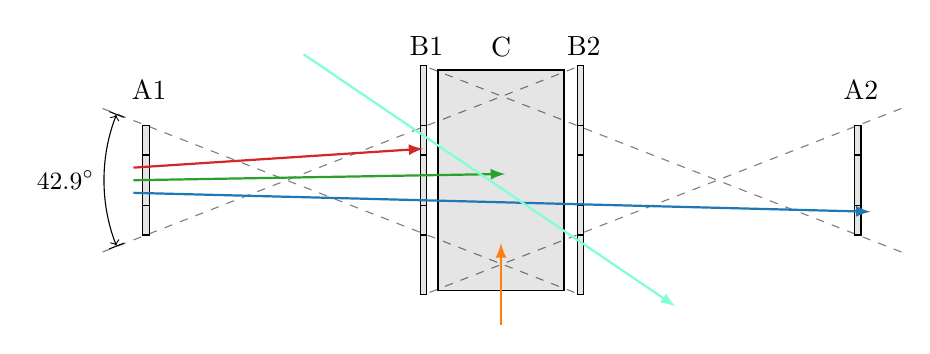
\begin{tikzpicture}[scale=0.8]
    \tikzset{%
        add/.style args={#1 and #2}{
            to path={%
                ($(\tikztostart)!-#1!(\tikztotarget)$)--($(\tikztotarget)!-#2!(\tikztostart)$)%
                \tikztonodes},add/.default={.2 and .2}}
    }   
    
    \def\Sithickness{0.05}
    
    % A1
    \draw[fill=light-gray] (-\Sithickness, -0.87) rectangle (\Sithickness, 0.87) node[above,yshift=2mm]{A1};
    \draw (-\Sithickness, -0.4) -- (\Sithickness, -0.4);
    \draw (-\Sithickness, 0.4) -- (\Sithickness, 0.4);
    
    % B1
    \draw[fill=light-gray] (4.4-\Sithickness, -1.82) rectangle (4.4+\Sithickness, 1.82) node[above]{B1};
    \draw (4.4-\Sithickness, -0.4) -- (4.4+\Sithickness, -0.4);
    \draw (4.4-\Sithickness, 0.4) -- (4.4+\Sithickness, 0.4);
    \draw (4.4-\Sithickness, -0.87) -- (4.4+\Sithickness, -0.87);
    \draw (4.4-\Sithickness, 0.87) -- (4.4+\Sithickness, 0.87);
    
    % C
    \draw[fill=light-gray] (4.635, -1.75) rectangle ++(2, 3.5);
    \node[above, yshift=0.5mm] at (5.635, 1.75) {C};
    
    % B2
    \draw[fill=light-gray] (6.9-\Sithickness, -1.82) rectangle (6.9+\Sithickness, 1.82) node[above]{B2};
    \draw (6.9-\Sithickness, -0.4) -- (6.9+\Sithickness, -0.4);
    \draw (6.9-\Sithickness, 0.4) -- (6.9+\Sithickness, 0.4);
    \draw (6.9-\Sithickness, -0.87) -- (6.9+\Sithickness, -0.87);
    \draw (6.9-\Sithickness, 0.87) -- (6.9+\Sithickness, 0.87);
    
    % A2
    \draw[fill=light-gray] (11.3-\Sithickness, -0.87) rectangle (11.3+\Sithickness, 0.87) node[above,yshift=2mm]{A2};
    \draw (11.3-\Sithickness, -0.4) -- (11.3+\Sithickness, -0.4);
    \draw (11.3-\Sithickness, 0.4) -- (11.3+\Sithickness, 0.4);
    
    % FOV
    \draw[add=0.1 and 0, dashed, opacity=0.5] (0, -0.87) to (6.9, 1.82);
    \draw[add=0.1 and 0, dashed, opacity=0.5] (0, 0.87) to (6.9, -1.82);
    \draw[add=0.1 and 0, dashed, opacity=0.5] (11.3, -0.87) to (4.4, 1.82);
    \draw[add=0.1 and 0, dashed, opacity=0.5] (11.3, 0.87) to (4.4, -1.82);
    
    \draw[|<->|] (0, 0.87) ++ (180-21.45:0.5) arc (180-21.45:180+21.45:2.4+0.48) node[midway, left] {\small\SI{42.9}{\degree}};
    

    \draw[thick, red, -latex] (-0.2, 0.2) -- (4.4, 0.5);
    \draw[thick, green, -latex] (-0.2, 0) -- (5.7, 0.1);
    \draw[thick, blue, -latex] (-0.2, -0.2) -- (11.5, -0.5);
    \draw[thick, Aquamarine, -latex] (2.5, 2) -- (8.4, -2);
    \draw[thick, orange, -latex] (5.635, -2.3) -- (5.635, -1);
\end{tikzpicture}
%\end{document}
        \end{column}
    \end{columns}
\end{frame}

\section{Statistical study of Forbush decreases at MSL/RAD}

\begin{frame}
    Inhalt...
\end{frame}

\section{Case study of the first CME observed at Solar Orbiter}

\begin{frame}
    Inhalt...
\end{frame}

\section{Conclusions and Outlook}

\begin{frame}
    Inhalt...
\end{frame}


\end{document}